\documentclass{article}
\usepackage{bm}
\usepackage{amssymb}
\usepackage{amsmath}
\usepackage[utf8]{inputenc}
\usepackage{hyperref}
\usepackage{xcolor}
\hypersetup{
    colorlinks=true,
    linkcolor=blue,
    filecolor=magenta,
    urlcolor=blue,
}
\usepackage{fullpage}
\usepackage{tikz}

\newcommand{\amy}[1]{{\color{blue}[Amy: #1]}}
\newcommand{\shekar}[1]{{\color{red}[Shekar: #1]}}
\newcommand{\matt}[1]{{\color{magenta}[Matt: #1]}}

\title{CSCI1410 Fall 2021 \\
Assignment 5: Reinforcement Learning}

\date{%
Code Submission 1 Due Thursday, November 4 at 11:59pm ET\\ [1ex]
Code Submission 2 Due Saturday, November 6 at 11:59pm ET\\ [1ex]
Code Due Monday, November 8 at 11:59pm ET\\ [1ex]
Writeup Due Tuesday, November 9 at 11:59pm ET\\ [1ex]
Late Day Deadline Thursday, November 11 at 11:59pm ET
}

\begin{document}

\maketitle


\section{Goals}
In this assignment, you will implement several variants of an
on-policy reinforcement learning (RL) algorithm called SARSA.  SARSA
stands for state-action-reward-state-action, as the algorithm updates
its $Q$-function at the current state and action based on its current
reward, its next state, and its next action.  This $Q$-function can be
represented by a table, indexed by states---themselves represented by
arbitrary (i.e., potentially non-linear) features---and actions.
Alternatively, it can be represented by an arbitrary function
approximator, in which case, the default representation is as a
``linear'' function of features and actions, which is approximated by
learning weights by which to linearly combine those features.%
\footnote{This second use of linear---linear combination---is what
  gives linear function approximation its name.}

The success of a reinforcement learning algorithm depends on the
settings of its multiple parameters: $\alpha$, $\gamma$, $\epsilon$,
$\lambda$, etc.  The process of optimizing these many parameters is
called \emph{hyper-parameter optimization}.  Because the search space
over parameter settings is vast (they generally cannot be optimized
independently), this process is usually automated.  Nonetheless, in
this assignment, you will experiment with just a few settings of these
parameters, which you will hand tune by inspecting learning curves.


\section{Silly Premise}
After weeks of a broken phone screen, George has finally decided to
drive over to the Apple store to get his screen fixed.  But by now,
his car is an autonomous reinforcement-learning agent, as are all the
taxis on the road!  George and his iPhone are thus at the mercy of how
well autonomous cars---which are piloted by RL---can drive.  As
George's car is stuck deep in a valley, he first attempts to get to
the Apple store via taxi.  Even if successful, he still has to get his
own car out of the valley.  Your RL algorithms will guide both his
taxi and his car.


\section{Overview}
This assignment has four parts:

\begin{enumerate}
    \item In the first part, you will implement SARSA and
      SARSA-$\lambda$ assuming a tabular representation of the
      $Q$-function to help navigate a taxi to its destination.
      
    \item In the second part, you will implement SARSA-$\lambda$
      assuming the $Q$-function is represented using a linear function
      approximator with Fourier basis functions to solve the mountain
      car problem, in which a car is stuck in a deep valley.
      
    \item In the third part, you will answer technical questions about
      RL.  You will also submit learning curves that vary with your
      hyperparameter settings, and summarize the results of your
      hyperparameter tuning.

    \item In the fourth part, you will answer ethics questions about RL.
\end{enumerate}

The coding portions of this assignment use
\href{https://openai.com/}{OpenAI}'s
\href{https://gym.openai.com/}{Gym}, an open source library with a
collection of RL tasks, for use in developing and benchmarking RL
algorithms.  Gym is written in Python, and includes multiple domains,
ranging from the classics (Acrobot, CartPole, Pendulum, Mountain Car,
etc.) to Atari games.  More details about Gym are provided in
Section~\ref{gym}.


\section{Taxi: SARSA and SARSA-$\lambda$}
In this problem, your goal is to help George get from a depot to the
Apple Store via taxi.  A sample taxi problem is depicted in
Figure~\ref{fig:taxi}.  It consists of a 5 $\times$ 5 grid, with four
designated pick-up and drop-off locations, R, G, B, and Y.

\begin{figure}[ht!]
  \centering
    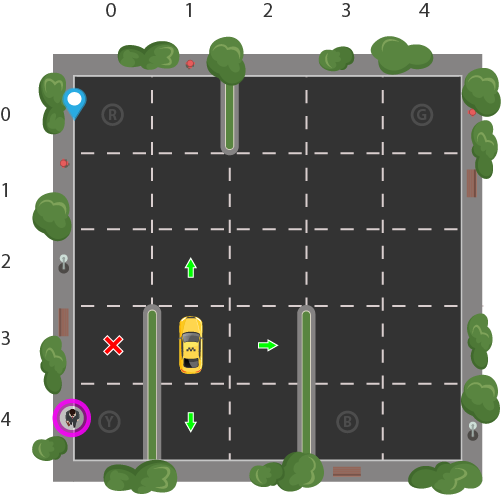
\includegraphics[width=2in]{taxi.png}
    \caption{A visualization of the taxi problem, in which a passenger is
      waiting to be picked up at Y ($(4,0)$) and dropped off at R ($(0,0)$).}
    \label{fig:taxi}
\end{figure}

As the \href{https://gym.openai.com/envs/Taxi-v2/}{taxi environment}
is available in Gym, you have been relieved of the task of
representing this problem as an MDP: i.e., of identifying the relevant
states and actions.  Still, before diving into the code, you should
spend a few minutes thinking about how you might have tackled this
representation problem.

Gym has also defined rewards for this problem somehow.  Intuitively,
the taxi should earn a high reward when George is picked up at his
location, and a very high reward when George is dropped off at the
Apple Store.  Additionally, it might make sense to penalize the taxi
for every step it takes, so that it doesn't drive around in circles
wasting gas.  Finally, it should also be heavily penalized if it drops
George off
%at the Android Store,% 
%\footnote{Is there such a place?}
%or
anywhere other than the Apple Store.  All of this information is
necessary to formulate the taxi problem as an MDP.

Just as the taxi can learn about its rewards by traversing its
environment, it can likewise learn about the transition probabilities.
Indeed, both transition probabilities and rewards are unknown.  If they
were known, the taxi could solve for an optimal policy using dynamic
programming.  But as this information is unknown, the taxi faces a
reinforcement learning problem.  Your job is to implement SARSA and
SARSA-$\lambda$, so the taxi can learn something close to an optimal
policy for picking up and dropping off passengers.


\subsection{Stencil Code}
Here, we briefly describe the primary functions in each file in the
taxi stencil code.  Please refer to comments in the code itself for
more details.  We also describe your specific coding tasks.

\begin{itemize}
\item \texttt{tabular\_sarsa.py}:
  This file contains the \texttt{Tabular\_SARSA} class,
  which is the parent class of the tabular SARSA classes that you will be implementing.
  It contains three data structures:
  \texttt{qtable} for storing state-action values,
  \texttt{etable} for storing eligibility values,
  and \texttt{policy} for storing a policy.
  It also contains a function called \texttt{learning\_policy}, which returns an optimal action,
  namely one that optimizes the $Q$-function.%
\footnote{In future versions of this assignment,
  \texttt{learning\_policy} will be renamed something more accurate like \texttt{choose\_action}.
Apologies for not making the change this year.  We did not want to risk breaking the autograder.}  
  \textbf{Do not edit this file.}

\item \texttt{taxi\_sarsa.py}:
  This file contains the \texttt{SARSA} class,
  within which you can find the \texttt{learn\_policy} function.
  This function takes as input all the relevant hyperparameters
  (e.g., $\alpha, \gamma, \epsilon, \lambda$, etc.),
  and returns a policy, a $Q$-function, and a sequence of rewards.
  Here is where you should implement the SARSA update rule.
  Doing so involves updating the \texttt{qtable}.

\item \texttt{taxi\_sarsa\_lambda.py}:
  Like \texttt{taxi\_sarsa.py}, this file contains another \texttt{SARSA} class,%
\footnote{In future versions of this assignment, we will not use the same name for two different classes.
Apologies for not making the change this year.  We did not want to risk breaking the autograder.}  
  within which you can again find a \texttt{learn\_policy} function.
  Again, this function takes as input all the relevant hyperparameters
  (e.g., $\alpha, \gamma, \epsilon, \lambda$, etc.),
  and returns a policy, a $Q$-function, and a sequence of rewards.
  Here is where you should implement the SARSA-$\lambda$ update rule.
  Doing so involves updating the \texttt{qtable} and the \texttt{etable}.
  
  \textbf{N.B.} Do not edit the \texttt{LearningPolicy} functions in
%either
  \texttt{taxi\_sarsa.py} or \texttt{taxi\_sarsa\_lambda.py}.
\footnote{In future versions of this assignment, we will not mix-and-match naming conventions.
We will follow a style guide, which will mean we either name all functions using a style like
\texttt{LearningPolicy}, or we will name all functions using a style like \texttt{learn\_policy}.
Apologies for not making this fix this year.  We did not want to risk breaking the autograder.}  
\end{itemize}


\subsection{Evaluation}
To test your code, you can run \texttt{python taxi\_sarsa.py test},
which executes your learned policy on multiple tasks, meaning multiple
different locations in which to pick George up and drop him off.  This
testing code outputs the total rewards earned on each task, and the
number of steps taken.  On average, your learned policy should
complete a task in fewer than 30 steps.

Running \texttt{python taxi\_sarsa.py test} also generates learning
curves, again averaged over multiple runs.  The $x$-axis of these
learning curves is the number of learning episodes (i.e., the number
of tasks on which the agent was trained), and the $y$-axis is the
total reward earned during that episode, averaged across the various
runs.  For SARSA, you should plot a learning curve over 1,000
episodes, and for SARSA-$\lambda$, 10,000.

You should also spend some, but not too much, time (e.g., 30 minutes)
hand-tuning the hyperparameters ($\alpha, \epsilon, \gamma, \lambda$,
etc.), before submitting two of your best learning curves with your
written handin.

The \texttt{test} argument to the \texttt{taxi\_sarsa.py} file
calls the \texttt{test\_policy} function, which
loads your policy from
\texttt{policy\_taxi\_sarsa\_grading.npy},
because that is the file name the autograder expects.
You thus have two choices when doing your own local testing:
either change the name of your output files to \\
\texttt{policy\_taxi\_sarsa\_grading.npy},
or change \texttt{test\_policy} to refer to
\texttt{policy\_taxi\_sarsa.npy} instead.

\textbf{N.B.}
Although the test code does not load the \texttt{qtable} (it relies
only on the \texttt{policy}), the autograder will check that the
\texttt{policy} you provide can be derived from the \texttt{qtable}
you provide, so be sure to submit two tables from the same run.

\vspace{2.5mm}

\textbf{A Note about Grading:}
The SARSA classes save the policy and state-action values to two
files, \texttt{policy\_taxi\_sarsa.npy} and
\texttt{qvalues\_taxi\_sarsa.npy}, respectively, for SARSA; likewise,
for SARSA-$\lambda$.  You must submit versions of these files from a
reasonable run for grading.  To do so, rename the saved files
\texttt{policy\_taxi\_sarsa\_grading.npy} and
\texttt{qvalues\_taxi\_sarsa\_grading.npy}, respectively; likewise,
for SARSA-$\lambda$.  The autograder will only grade these renamed
files.


\section{Mountain-car}
George's car is stuck at the bottom of a valley.  The Apple store,
however, is at the top of the mountain, marked with a green flag.
Figure~\ref{fig:mountain_car} depicts this domain.

\begin{figure}[ht!]
    \centering
    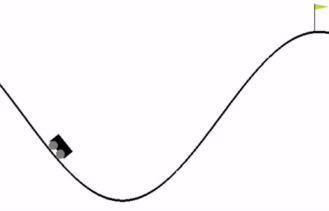
\includegraphics[width=2in]{mountain_car.png}
    \caption{A visualization of the mountain car problem.}
    \label{fig:mountain_car}
\end{figure}

The car does not have enough power to just drive up the hill.
Instead, it needs to rock back and forth until it gains enough
momentum.  So, it's actions are move left, move right, and skip (i.e.,
do nothing).

The car's state space $S$ is continuous.  It consists of two
real-values, namely the car's position along the $x$-axis and its
velocity.  Since $S = \mathbb{R}^2$, we cannot represent the
$Q$-function for mountain car as a table.  Instead, we will use a
linear function approximator.

We start by representing the state-value function $V$ using a linear
function approximator.  To do so, we choose a set of $n$ basis
functions, $\phi_i: S \to \mathbb{R}^{m}$, for $i \in \{ 1, \ldots, n
\}$, each of which maps a state $s \in S$ onto an $m$-dimensional
basis.  We then define the $V$-function to be a weighted combination
of these basis functions: i.e., for weights $\bm{w} \in \mathbb{R}^m$,
\begin{equation}
V(s) = \sum_{i = 1}^{n} w_i \phi_i (s) \enspace
\end{equation}
Therefore, 
\begin{align}
Q(s,a)
&= R(s,a) + \gamma \mathbb{E}_{s' \in S} \left[ V (s') \right] \\
&= R(s,a) + \gamma \mathbb{E}_{s' \in S} \left[ \sum_{i = 1}^{n} w_i \phi_i (s') \right] \enspace
\end{align}

For this assignment, we recommend the Fourier basis.  The univariate
$n$th order Fourier basis consists of $n+1$ basis functions defined as
follows: $\phi_i(x) = \cos (\pi i x)$, for $i \in \{ 0, \ldots, n \}$
and $x \in S$.  For a multi-dimensional state space, such as that of
the mountain car problem, where the number of dimensions $d = 2$, the
$n$th order Fourier basis consists of $(n+1)^d$ basis functions
defined as follows: $\phi_i(\bm{x}) = \cos (\pi \bm{c}^i \cdot
\bm{x})$, for all $i \in \{ 0, \ldots, (n+1)^d \}$ and $\bm{x} \in S$,
where the $\bm{c}$ vectors range over all $d$-dimensional vectors in
$\{ 0, \ldots, n+1 \}^d$.  For more details and motivation for the
Fourier basis, we refer you to
\href{http://cs.brown.edu/people/gdk/pubs/fourier.pdf}{a paper by
  George himself}.

Like the taxi, the mountain car would like to execute an optimal
policy.  Again, the rewards and transitions are unknown; only a
simulator is provided (within Gym).  So the mountain car faces a
reinforcement learning problem.  Your job is to implement
SARSA-$\lambda$ with function approximation, so the mountain car can
learn something close to an optimal policy.  Pseudocode for
SARSA-$\lambda$ can be found in this
\href{http://incompleteideas.net/book/first/ebook/node89.html}{online
  RL textbook}.


\subsection{Stencil Code}
Here, we briefly describe the primary functions in
\texttt{mountain\_car\_sarsa\_fourier.py}.  Please refer to comments
in the code itself for more details.  We also describe your specific
coding tasks.

\textbf{Please do not modify any functions except those you are
  explicitly instructed to modify.}

\begin{enumerate}
\item \texttt{normalize\_state}: This function normalizes each
  dimension of the state (position and velocity) to lie within the
  range $[0,1]$. Normalization is not strictly necessary, as the
  weights may be adjusted to account for any differences in magnitude
  among the various state dimensions, but it does simplify and often
  speed up the learning process.
  
\item \texttt{phi}: This function takes in a normalized state and
  computes its value, given a basis. \textbf{You need to fill in this
    function.}
  
\item \texttt{create\_multipliers}: This function creates the Fourier
  basis coefficients (i.e., the $\bm{c}$ vectors). \textbf{You need to
    fill in this function.}
  
\item \texttt{action\_value}: This function returns an action value,
  given a state-action pair.
  
\item \texttt{learning\_policy} and \texttt{test\_policy}: These
  functions return an optimal action, given a state, with and without
  exploration, respectively.  If an agent is no longer learning, it
  need not need explore any further either; hence, a separate function.%
\footnote{This is poor programming practice.  Can you see why?  Because there should not
  be two functions where one (\texttt{test\_policy}) is a special case of the other (\texttt{learn\_policy}).
  In future versions of this assignment, \texttt{test\_policy} will be defined as \texttt{learn\_policy} with epsilon fixed at 0,
  to prevent exploration.}
  
\item \texttt{SARSA\_Learning}: This function should update the
  weights associated with the basis functions using the
  SARSA-$\lambda$ algorithm.  Some of the function is filled in for
  you, to interface to the rest of the code, but \textbf{you need to
    fill in the rest.}

\item \texttt{SARSA\_Test}: This function uses the weights learned or
  saved to act over a specified number of episodes.  You can run this
  function to test your policy before you submit it.
\end{enumerate}


\subsection{Evaluation}
To test your code, you can run \texttt{python
  mountain\_car\_sarsa\_fourier.py test}, which executes your learned
policy multiple times.  This testing code outputs the total rewards
earned on each execution, and the number of steps taken.  On average,
your learned policy should complete the task in fewer than 400 steps.

Running \texttt{python mountain\_car\_sarsa\_fourier.py test} also
generates learning curves,%
\footnote{Actually, it does not---unfortunately---but it should. For
  extra credit, please go ahead and adjust the test code so that it
  does generate plots, so that you can more easily tune the
  hyperparameters of your implementation.} again averaged over
multiple runs.  The $x$-axis of these learning curves is the number of
learning episodes (i.e., the number of tasks on which the agent was
trained), and the $y$-axis is the total reward earned during that
episode, averaged across the various runs.  You should plot a learning
curve over 10,000 episodes.

You should also spend some, but not too much, time (e.g., 30 minutes)
hand-tuning the hyperparameters ($\alpha, \epsilon, \gamma, \lambda$,
etc.), before submitting one of your best learning curves with your
written handin.

Note that order of the Fourier basis is an important parameter.  We
initialized this value to 3.  It should remain odd (e.g., 1, 5, 7,
etc.), but you should otherwise feel free to experiment with alternatives.

The \texttt{test} argument to the
\texttt{mountain\_car\_sarsa\_fourier.py} \\
file loads your policy from
\texttt{policy\_mountain\_car\_saved\_weights.npy}. \\
\emph{This time, that is not the name the autograder expects!}
(Apologies for the inconsistencies in this assignment.)

\vspace{2.5mm}

\textbf{A Note about Grading:}
The \texttt{SARSA\_Learning} function saves the learned weights to a
file called \texttt{mountain\_car\_saved\_weights.npy}.  You must
submit a version of this file from a reasonable run for grading.  To
do so, rename the saved file
\texttt{mountain\_car\_saved\_weights\_grading.npy}.  The autograder
will only grade a file by this latter name.


\section{Written Questions}
Answer the following questions in clearly labeled sections.

\begin{enumerate}

\item
  Describe any possible state space representation for the taxi environment
  (even the one used in Gym).
  
\if 0
The first component of the state space is the taxi's location,
which can be represented as
a pair.  For example, in Figure~\ref{fig:taxi}, the taxi is located at
$(3,1)$.  As the domain is a 5 $\times$ 5 grid, there are 25 possible taxi locations.
%
Second is the passenger's location, of which there are 4 possibilities
at the start---R, G, B, and Y, located at $(0,0), (0,4), (4,3)$, and
$(4,0)$, respectively---plus the additional possibility of ``being
transported,'' for a total of 5 possible states.
%
Finally, there are four possibilities for the passenger's goal: again,
R, G, B, and Y.
%
Thus, in total, there are 500 = 25 $\times$ 5 $\times$ 4 states.

As for available actions, the taxi can move north, south, east, or
west, and it can pick up or drop off George.
\fi

\item
  Submit your learning curves, and explain what you gleaned from them.
  What settings of the hyperparameters did you find worked best in the taxi problem?
  And what about in mountain car?%
\footnote{For extra credit, you may submit learning curves for mountain car as well as the taxi problem.
You are also permitted to post your plotting code on Piazza, as that would be a help to your fellow students.
Please let Amy know if you do this, so that she can award you good Samaritan points (and can recommend you as a TA for next year!).}
  What happened when you changed the order of the Fourier basis?

\item
  Recall that Arthur Samuel used machine learning back in 1959 to
  train his checker-playing program.  More relevant this assignment,
  in 1992 Gerry Tesauro, used \emph{reinforcement learning\/} with
  (non-linear) function approximation in his award-winning
  backgammon-playing program, TD-Gammon.%
  \footnote{Now you know what ``TD'' means! Hurray!}
  In both cases, the programs improved their play (i.e., learned)
  by playing against themselves.
  
  How can you formulate learning to play a two-player game, like
  backgammon or Go,
%in self-play (i.e., against yourself)
  as an MDP?  What are the states, the actions, the rewards, and the
  transitions?  And why does it make more sense to formulate such a
  problem as a reinforcement learning problem, in which rewards and
  transitions are unknown to the learning agent, rather than attempt
  to solve such an MDP via dynamic programming?
\end{enumerate}

\if 0
\item
  
\begin{enumerate}
\item Probabilistic Planning problems and Reinforcement Learning
  problems have a lot in common; However, there is a fundamental
  difference between these two types of problems. What is that
  difference? In other words, what determines if a problem is a
  Probabilistic Planning problem or a Reinforcement Learning problem?
  Your answer should be one or two sentences.

\item Discuss at least one important consequence of this difference,
  as it applies to solving the problems.

\item Give an example of a probabilistic planning problem. Modify it
  slightly to create a reinforcement learning problem.  
\end{enumerate}

\item Suppose you have a reinforcement learning agent that learns an
  estimate of the action-value (Q) function of its environment and
  then uses its estimate to choose actions.

  When the agent uses its estimate of the Q-function to choose an
  action at state $s$, it faces a tradeoff: it can choose the action
  that appears to be best under its estimate, $a^* \equiv arg\max_a
  {Q(s, a)}$, or it can choose a different action $a_e \neq a^*$, in
  hopes of improving its estimate of $Q(s, a_e)$, since doing so may
  increase the sum of discounted reward in the long run. What is
  this tradeoff called, and what is one way that your agent could
  manage it effectively?
\fi
    

\section{Ethics Questions}
Read the article \href{https://www.fast.ai/2021/07/19/copilot/}{here} about Github Copilot. Github Copilot is Github's recent invite-only to use tool for to assist programmers. Github copilot is partially based on an NLP model from GPT-3, which was partially trained using reinforcement learning. It is trained using open source repositories on Github. Please read the following article on Github Copilot and answer the following questions:
\begin{enumerate}
    \item Should Github be required to aquire the explicit consent of the contributors to open source repositories to use their code as training data for Copilot. In general. should explicit consent be required to use open source data?
    \item If sensitive data such as API keys are leaked by Github Copilot AI is it the responsibility of Github to prevent that or is it the responsibility of the original creators of the code to make that sensitive information more secure. Or another party entirely?
\end{enumerate}



\section{Gym Installation}
\label{gym}

There are several packages that are needed for this project.  Some of
the necessary packages are: \texttt{gym}, \texttt{matplotlib}, and
\texttt{numpy}.  If you use the course virtual environment you
shouldn't need to install anything, but if you are working locally you
may need to install these by running \texttt{pip install `gym[all]'}.
%
Additionally, here are two tutorials that explain how to use AI gym to
solve the
\href{https://towardsdatascience.com/reinforcement-learning-lets-teach-a-taxi-cab-how-to-drive-4fd1a0d00529}{taxi}
and  
\href{https://towardsdatascience.com/getting-started-with-reinforcement-learning-and-open-ai-gym-c289aca874f}{mountain car}
problems.%
\footnote{We cannot vouch for their accuracy.  There are many tutorials out there.
  If you find better ones, please share on Piazza.}


\section{Grading}
As usual, you can refer to \verb|rubric.txt| to see how heavily each
part of this assignment is weighted.

We will autograde the output of your SARSA and SARSA-$\lambda$
implementations for the taxi problem using the files you submit,
containing your learned policy and $Q$-values.  We will simulate your
policy on 10 random tasks, and award you full points if the average number
of steps to completion is under $30$.

We will also autograde the output of your SARSA-$\lambda$
implementation for mountain car using the file you submit, containing
your learned weights.  Again, we will simulate your policy 10 times,
but as mountain car is a harder problem, we will award you full points
if the average number of steps to completion is under $400$.

In all cases, the time limit for each test run is 30 seconds.  In
other words, if ever your policy does not complete a task within
this time limit, you will score 0 on that test run.
%\amy{what happens? is your score for that task 0?}
%\matt{historically yes. Earlier in the year, we had concerns over a slow autograder so we will talk to HTAs on how best to adjust this policy}

In addition to the aforementioned autograding, we will also verify
that your submitted code corresponds to your submitted data files and
learning curves.  \textbf{If we find that the data files and/or the
  learning curves that you submit could not have been generated by
  your code, you will earn a zero for the entire assignment.}

\textbf{Note:} After generating your \texttt{.npy} files, you need to rename
them by appending \texttt{$\_$grading.npy} to the end of each file name.
Incorrectly named files will not be graded.


\section{Install and Handin Instructions}
To install, accept the GitHub Classroom assignment at \href{https://classroom.github.com/a/go7hYD7v}{this link}. This will
create a private GitHub repository with the stencil code for you to work on the
assignment.

To handin,
\begin{enumerate}
  \item Make sure to push any changes you want to test to your private
    repository. You can do this by running
    \begin{verbatim}
    git add .
    git commit -m "<a commit message describing what you changed>"
    git push
    \end{verbatim}

  \item On Gradescope, click on the assignment you are submitting for.

  \item Under ``Submission Method", please select GitHub.

  \item Under ``Repository", you can search for your repository by typing ``csci-1410"
    and selecting the repository for this assignment.

  \item Under ``Branch", you can select any branch that you want to be graded. So if
    you're testing something on a branch, you can see how its functionality
    performs here, before merging it to master. Feel free to upload your assignment
    as many times as you like before the deadline.
\end{enumerate}

In accordance with the course \href {https://cs1410-website.vercel.app/files/Collaboration_Policy.pdf}{grading policy},
your written homework should not have any identifiable information on it,
including your banner ID, name, or CS login.

\end{document}


\end{document}
